\documentclass[twocolumn]{article}
\usepackage{graphicx}
\title{\vspace{-3.5cm}The Fresnel integrals and the Euler curve}
\author{S.H.~Albrechtsen}

\begin{document}
\maketitle
All information in this text is taken from Wikipedia\cite{WikiFresnelIntegral}.
\section{The Fresnel integrals}
The Frenel Integrals are two trandenceltal functions used in optics. They are defined by the following integrals:
\begin{equation}
S(x) = \int_{0}^{x} \sin(t^2) dt\label{eq:S} \textrm{, and}
\end{equation}
\begin{equation}
C(x) = \int_{0}^{x} \cos(t^2) dt\label{eq:C},
\end{equation}
and appear in the discription of near-field Fresnel diffraction. A plot of the integrals can be seen in figure \ref{fig:SandC}.

\begin{figure}
\centering
% GNUPLOT: LaTeX picture with Postscript
\begingroup
  \makeatletter
  \providecommand\color[2][]{%
    \GenericError{(gnuplot) \space\space\space\@spaces}{%
      Package color not loaded in conjunction with
      terminal option `colourtext'%
    }{See the gnuplot documentation for explanation.%
    }{Either use 'blacktext' in gnuplot or load the package
      color.sty in LaTeX.}%
    \renewcommand\color[2][]{}%
  }%
  \providecommand\includegraphics[2][]{%
    \GenericError{(gnuplot) \space\space\space\@spaces}{%
      Package graphicx or graphics not loaded%
    }{See the gnuplot documentation for explanation.%
    }{The gnuplot epslatex terminal needs graphicx.sty or graphics.sty.}%
    \renewcommand\includegraphics[2][]{}%
  }%
  \providecommand\rotatebox[2]{#2}%
  \@ifundefined{ifGPcolor}{%
    \newif\ifGPcolor
    \GPcolortrue
  }{}%
  \@ifundefined{ifGPblacktext}{%
    \newif\ifGPblacktext
    \GPblacktexttrue
  }{}%
  % define a \g@addto@macro without @ in the name:
  \let\gplgaddtomacro\g@addto@macro
  % define empty templates for all commands taking text:
  \gdef\gplbacktext{}%
  \gdef\gplfronttext{}%
  \makeatother
  \ifGPblacktext
    % no textcolor at all
    \def\colorrgb#1{}%
    \def\colorgray#1{}%
  \else
    % gray or color?
    \ifGPcolor
      \def\colorrgb#1{\color[rgb]{#1}}%
      \def\colorgray#1{\color[gray]{#1}}%
      \expandafter\def\csname LTw\endcsname{\color{white}}%
      \expandafter\def\csname LTb\endcsname{\color{black}}%
      \expandafter\def\csname LTa\endcsname{\color{black}}%
      \expandafter\def\csname LT0\endcsname{\color[rgb]{1,0,0}}%
      \expandafter\def\csname LT1\endcsname{\color[rgb]{0,1,0}}%
      \expandafter\def\csname LT2\endcsname{\color[rgb]{0,0,1}}%
      \expandafter\def\csname LT3\endcsname{\color[rgb]{1,0,1}}%
      \expandafter\def\csname LT4\endcsname{\color[rgb]{0,1,1}}%
      \expandafter\def\csname LT5\endcsname{\color[rgb]{1,1,0}}%
      \expandafter\def\csname LT6\endcsname{\color[rgb]{0,0,0}}%
      \expandafter\def\csname LT7\endcsname{\color[rgb]{1,0.3,0}}%
      \expandafter\def\csname LT8\endcsname{\color[rgb]{0.5,0.5,0.5}}%
    \else
      % gray
      \def\colorrgb#1{\color{black}}%
      \def\colorgray#1{\color[gray]{#1}}%
      \expandafter\def\csname LTw\endcsname{\color{white}}%
      \expandafter\def\csname LTb\endcsname{\color{black}}%
      \expandafter\def\csname LTa\endcsname{\color{black}}%
      \expandafter\def\csname LT0\endcsname{\color{black}}%
      \expandafter\def\csname LT1\endcsname{\color{black}}%
      \expandafter\def\csname LT2\endcsname{\color{black}}%
      \expandafter\def\csname LT3\endcsname{\color{black}}%
      \expandafter\def\csname LT4\endcsname{\color{black}}%
      \expandafter\def\csname LT5\endcsname{\color{black}}%
      \expandafter\def\csname LT6\endcsname{\color{black}}%
      \expandafter\def\csname LT7\endcsname{\color{black}}%
      \expandafter\def\csname LT8\endcsname{\color{black}}%
    \fi
  \fi
    \setlength{\unitlength}{0.0500bp}%
    \ifx\gptboxheight\undefined%
      \newlength{\gptboxheight}%
      \newlength{\gptboxwidth}%
      \newsavebox{\gptboxtext}%
    \fi%
    \setlength{\fboxrule}{0.5pt}%
    \setlength{\fboxsep}{1pt}%
\begin{picture}(4520.00,2820.00)%
    \gplgaddtomacro\gplbacktext{%
      \csname LTb\endcsname%%
      \put(747,865){\makebox(0,0)[r]{\strut{}$-0.8$}}%
      \csname LTb\endcsname%%
      \put(747,1258){\makebox(0,0)[r]{\strut{}$-0.4$}}%
      \csname LTb\endcsname%%
      \put(747,1651){\makebox(0,0)[r]{\strut{}$0$}}%
      \csname LTb\endcsname%%
      \put(747,2044){\makebox(0,0)[r]{\strut{}$0.4$}}%
      \csname LTb\endcsname%%
      \put(747,2437){\makebox(0,0)[r]{\strut{}$0.8$}}%
      \csname LTb\endcsname%%
      \put(1084,409){\makebox(0,0){\strut{}$-9$}}%
      \csname LTb\endcsname%%
      \put(1566,409){\makebox(0,0){\strut{}$-6$}}%
      \csname LTb\endcsname%%
      \put(2049,409){\makebox(0,0){\strut{}$-3$}}%
      \csname LTb\endcsname%%
      \put(2531,409){\makebox(0,0){\strut{}$0$}}%
      \csname LTb\endcsname%%
      \put(3013,409){\makebox(0,0){\strut{}$3$}}%
      \csname LTb\endcsname%%
      \put(3496,409){\makebox(0,0){\strut{}$6$}}%
      \csname LTb\endcsname%%
      \put(3978,409){\makebox(0,0){\strut{}$9$}}%
    }%
    \gplgaddtomacro\gplfronttext{%
      \csname LTb\endcsname%%
      \put(153,1651){\rotatebox{-270}{\makebox(0,0){\strut{}$y$}}}%
      \csname LTb\endcsname%%
      \put(2531,130){\makebox(0,0){\strut{}$x$}}%
      \csname LTb\endcsname%%
      \put(3351,1022){\makebox(0,0)[r]{\strut{}$\mathrm{S}(x)$}}%
      \csname LTb\endcsname%%
      \put(3351,836){\makebox(0,0)[r]{\strut{}$\mathrm{C}(x)$}}%
    }%
    \gplbacktext
    \put(0,0){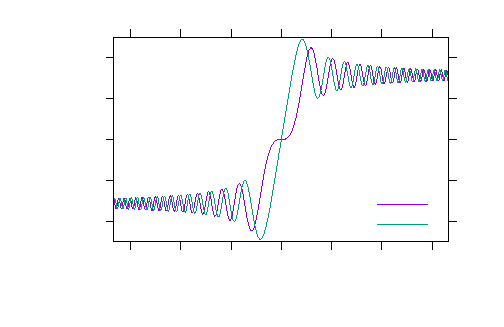
\includegraphics{plot-SandC}}%
    \gplfronttext
  \end{picture}%
\endgroup

\caption{The $S(x)$ and $C(x)$ functions.\label{fig:SandC}}
\end{figure}

As an alternative to equation \ref{eq:S} and \ref{eq:C}, the functions can be computed by the power series expansion, which converges for all x:
\begin{equation}\label{eq:SPowerSeries}
S(x) = \sum_{n=0}^{\infty}(-1)^n\frac{x^{4n+3}}{(2n+1)!(4n+3)}.
\end{equation}
\begin{equation}\label{eq:CPowerSeries}
C(x) = \sum_{n=0}^{\infty}(-1)^n\frac{x^{4n+1}}{(2n)!(4n+1)}.
\end{equation}

\section{Mathematical properties}
\begin{itemize}
\item Both of the Fresnel integrals are odd functions of their parameter $x$.
\item Using the power series, see equation \ref{eq:SPowerSeries} and \ref{wq:CPowerSeries}, the Fresnel integrals can be extended to the complex plane.
\item In the limit of $x$ going to infinity: $C(\infty) = S(\infty) = \sqrt{\frac{\pi}{8}}\approx0.6267$
\end{itemize}

\section{The Euler Spiral}
The following parametric function is called the Euler spiral, and is plottet in figure \ref{fig:eulerSpiral}
\begin{equation}
(x, y) = (C(t), S(t)).
\end{equation}

The euler spiral has the mathematical property that the curvature at any point is proportional to the length of the spiral, measured from the origin. Thereby, a vehicle following the spiral at a constant speed will experince a constant rate of angular acceleration.

\begin{figure}
\centering
% GNUPLOT: LaTeX picture with Postscript
\begingroup
  \makeatletter
  \providecommand\color[2][]{%
    \GenericError{(gnuplot) \space\space\space\@spaces}{%
      Package color not loaded in conjunction with
      terminal option `colourtext'%
    }{See the gnuplot documentation for explanation.%
    }{Either use 'blacktext' in gnuplot or load the package
      color.sty in LaTeX.}%
    \renewcommand\color[2][]{}%
  }%
  \providecommand\includegraphics[2][]{%
    \GenericError{(gnuplot) \space\space\space\@spaces}{%
      Package graphicx or graphics not loaded%
    }{See the gnuplot documentation for explanation.%
    }{The gnuplot epslatex terminal needs graphicx.sty or graphics.sty.}%
    \renewcommand\includegraphics[2][]{}%
  }%
  \providecommand\rotatebox[2]{#2}%
  \@ifundefined{ifGPcolor}{%
    \newif\ifGPcolor
    \GPcolortrue
  }{}%
  \@ifundefined{ifGPblacktext}{%
    \newif\ifGPblacktext
    \GPblacktexttrue
  }{}%
  % define a \g@addto@macro without @ in the name:
  \let\gplgaddtomacro\g@addto@macro
  % define empty templates for all commands taking text:
  \gdef\gplbacktext{}%
  \gdef\gplfronttext{}%
  \makeatother
  \ifGPblacktext
    % no textcolor at all
    \def\colorrgb#1{}%
    \def\colorgray#1{}%
  \else
    % gray or color?
    \ifGPcolor
      \def\colorrgb#1{\color[rgb]{#1}}%
      \def\colorgray#1{\color[gray]{#1}}%
      \expandafter\def\csname LTw\endcsname{\color{white}}%
      \expandafter\def\csname LTb\endcsname{\color{black}}%
      \expandafter\def\csname LTa\endcsname{\color{black}}%
      \expandafter\def\csname LT0\endcsname{\color[rgb]{1,0,0}}%
      \expandafter\def\csname LT1\endcsname{\color[rgb]{0,1,0}}%
      \expandafter\def\csname LT2\endcsname{\color[rgb]{0,0,1}}%
      \expandafter\def\csname LT3\endcsname{\color[rgb]{1,0,1}}%
      \expandafter\def\csname LT4\endcsname{\color[rgb]{0,1,1}}%
      \expandafter\def\csname LT5\endcsname{\color[rgb]{1,1,0}}%
      \expandafter\def\csname LT6\endcsname{\color[rgb]{0,0,0}}%
      \expandafter\def\csname LT7\endcsname{\color[rgb]{1,0.3,0}}%
      \expandafter\def\csname LT8\endcsname{\color[rgb]{0.5,0.5,0.5}}%
    \else
      % gray
      \def\colorrgb#1{\color{black}}%
      \def\colorgray#1{\color[gray]{#1}}%
      \expandafter\def\csname LTw\endcsname{\color{white}}%
      \expandafter\def\csname LTb\endcsname{\color{black}}%
      \expandafter\def\csname LTa\endcsname{\color{black}}%
      \expandafter\def\csname LT0\endcsname{\color{black}}%
      \expandafter\def\csname LT1\endcsname{\color{black}}%
      \expandafter\def\csname LT2\endcsname{\color{black}}%
      \expandafter\def\csname LT3\endcsname{\color{black}}%
      \expandafter\def\csname LT4\endcsname{\color{black}}%
      \expandafter\def\csname LT5\endcsname{\color{black}}%
      \expandafter\def\csname LT6\endcsname{\color{black}}%
      \expandafter\def\csname LT7\endcsname{\color{black}}%
      \expandafter\def\csname LT8\endcsname{\color{black}}%
    \fi
  \fi
    \setlength{\unitlength}{0.0500bp}%
    \ifx\gptboxheight\undefined%
      \newlength{\gptboxheight}%
      \newlength{\gptboxwidth}%
      \newsavebox{\gptboxtext}%
    \fi%
    \setlength{\fboxrule}{0.5pt}%
    \setlength{\fboxsep}{1pt}%
\begin{picture}(3960.00,3400.00)%
    \gplgaddtomacro\gplbacktext{%
      \csname LTb\endcsname%%
      \put(803,669){\makebox(0,0)[r]{\strut{}$-1$}}%
      \csname LTb\endcsname%%
      \put(803,1305){\makebox(0,0)[r]{\strut{}$-0.5$}}%
      \csname LTb\endcsname%%
      \put(803,1941){\makebox(0,0)[r]{\strut{}$0$}}%
      \csname LTb\endcsname%%
      \put(803,2577){\makebox(0,0)[r]{\strut{}$0.5$}}%
      \csname LTb\endcsname%%
      \put(803,3213){\makebox(0,0)[r]{\strut{}$1$}}%
      \csname LTb\endcsname%%
      \put(979,409){\makebox(0,0){\strut{}$-1$}}%
      \csname LTb\endcsname%%
      \put(1615,409){\makebox(0,0){\strut{}$-0.5$}}%
      \csname LTb\endcsname%%
      \put(2251,409){\makebox(0,0){\strut{}$0$}}%
      \csname LTb\endcsname%%
      \put(2887,409){\makebox(0,0){\strut{}$0.5$}}%
      \csname LTb\endcsname%%
      \put(3523,409){\makebox(0,0){\strut{}$1$}}%
    }%
    \gplgaddtomacro\gplfronttext{%
      \csname LTb\endcsname%%
      \put(209,1941){\rotatebox{-270}{\makebox(0,0){\strut{}$S(x)$}}}%
      \csname LTb\endcsname%%
      \put(2251,130){\makebox(0,0){\strut{}$C(x)$}}%
      \csname LTb\endcsname%%
      \put(2735,836){\makebox(0,0)[r]{\strut{}Euler curve}}%
    }%
    \gplbacktext
    \put(0,0){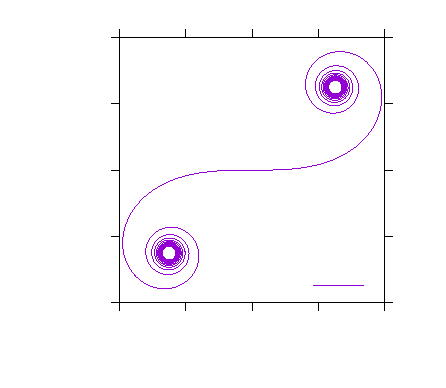
\includegraphics{plot-euler}}%
    \gplfronttext
  \end{picture}%
\endgroup

\caption{The euler curve for for a parameteri $t$ in the interval $[-10, 10]$.\label{fig:eulerSpiral}}
\end{figure}

\bibliography{references}{}
\bibliographystyle{plain}

\end{document}
